\chapter{Introdución}
\label{chap:introducion}
\section{Obxetivos}
Este proxecto consiste en elaborar un xogo para o sistema operativo \textbf{Android} \cite{android-dev} \cite{night-mode} \cite{landscape} \cite{start-activity} basado no tradicional xogo do \textbf{Forcado}. O obxetivo da aplicación é poder xogar de maneira \textbf{individual} ou \textbf{multixogador} tratando de adiviñar a palabra secreta antes de que se forme por completo o forcado.\\
\\
A aplicación estará enfocada ao xogo en local, é dicir, desde un único dispositivo aínda que contaremos cunha versión multixogador online ao final do proxecto. Implementarase un dicionario ao que o usuario lle pode engadir palabras e serían candidatas a ser seleccionadas aleatoriamente para ter que adiviñalas nunha partida.

\section{Motivación}
Visto o auxe do xénero do videoxogo na vida cotiá e a utilización de dispositivos móbiles estendidos cada vez máis en distintos rangos de idades dos usuarios decidimos decantarnos por implementar un videoxogo para dispositivo móbil sinxelo, fácil de utilizar, entendible e apto para todo tipo de público.


\section{Traballo relacionado}
Hai diversas aplicacións na Play Store nas que desenvolveron o mesmo xogo.
As dúas con maior impacto a nivel de descargas (> 10 millóns). Ambas aplicacións amosan unha interface familiar e intuitiva, podemos tomar como comparativa estas dúas aplicacións para partir do deseño, xa que este videoxogo en concreto non ofrecen moitas posibilidades neste aspecto. Nas que nos estamos baseando, son as seguintes:\\[100 pt]
\href{https://play.google.com/store/apps/details?id=com.tellmewow.senior.hangman&hl=es&gl=US}{Ahorcado desarrollado por Senior Games:}\\
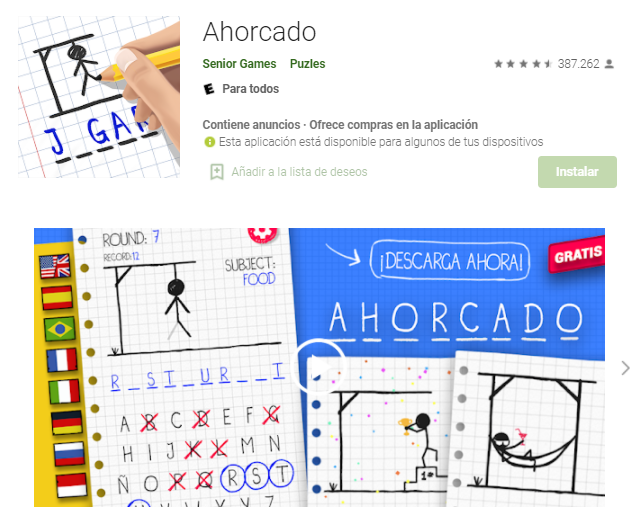
\includegraphics[scale=0.65]{imaxes/app1.png}\\[12 pt]

\href{https://play.google.com/store/apps/details?id=com.quarzo.hangmanwords&hl=es&gl=US}{Ahorcado desarrollado por Quarzo Apps:}\\
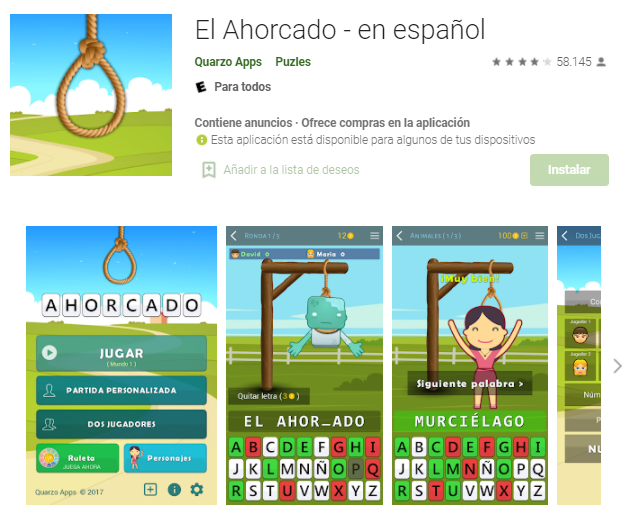
\includegraphics[scale=0.65]{imaxes/app2.png}\\[12 pt]
 \let\cleardoublepage=\clearpage 
 
 

